\chapter{A framework to improve Ceccato et al.’s work.}
\label{proposal}

\linenumbers
\lettrine[lines=2]{I}{n Chapter \ref{state_of_art}}, I presented the state of the art of \textit{process comprehension} of an Industrial Control System (ICS) focusing later on the methodology proposed by Ceccato et al. \cite{ceccato}[Section \ref{sec:ceccato_metodology}], explaining what it consists of, its practical application on a testbed, and most importantly highlighting its limitations and critical issues (see Section \ref{subsec:ceccato_limitations}).

\bigskip
In this chapter I will present \textbf{my proposals to improve the methodology} presented in the previous chapter, overcoming (or at least trying to do so) the criticalities mentioned above by almost completely rewriting the original framework, enhancing its functionalities and inserting new ones where possible, while keeping its general structure and approach: the system analysis will in fact consist of the same four steps as in the original methodology (Data Pre-processing, Graph and Statistical Analysis, Business Process Mining and Invariants Inference), but each of them will be deeply revised in order to provide a richer, clearer and more complete process comprehension of the industrial system to be analyzed and its behavior.

\bigskip
As it may have already been noted, my proposals do not involve improving the data gathering phase: this is due simply to the fact that the novel framework will not be tested on the same case study used by Ceccato et, al. (Section \ref{subsec:ceccato_testbed}), but on a different case study, the ITrust SWaT system \cite{swat_home}, of which (some) datasets containing the execution trace of the physical system and the network traffic scan are already provided by iTrust itself. For more details about this case study, see Chapter \ref{casestudy}.

\section{The novel Framework}
\label{sec:4_framework_presentation}
The implementation of the novel framework for ICSs analysis starts from several assumptions:

\begin{enumerate}
	\item it must be implemented in a \textbf{single programming language}
	\item it must be \textbf{independent of the system} to be analyzed
	\item It must provide greater \textbf{flexibility and ease of use} for the user at every stage
\end{enumerate}
In the following, these three points will be discussed in more detail.

\begin{description}
	\item[Single Programming Language] The original tool was implemented using various programming languages in each of the different phases: from Python up to Java, passing through Bash scripting. \newline
	In my opinion, this heterogeneity makes it more difficult and less intuitive for the user to operate on the tool: moreover, the use of multiple technologies makes it more difficult to maintain the code and add new features, particularly if only a single person is managing the code (he/she might be proficient in one language, but little of the others).
	
	\bigskip
	For these reasons, I decided to use a single programming language, to ensure homogeneity to the framework and ease of use and maintenance of the code for anyone who wants to manage it in the future: I chose to use Python, because of its simplicity and easy readability combined with its versatility and powerfulness: moreover, Python can count on a massive number of available libraries and packages that meet all kinds of needs.
	
	\item[System Independence] One of the biggest limitations of Ceccato et al.'s tool that I highlighted in Section \ref{subsec:ceccato_limitations} is the fact that it is \textbf{highly dependent on the testbed used}: that is, it is \textit{not} possible to configure any of the tool's parameters to analyze different industrial systems.\newline
	To overcome this issue and make my framework independent of the system to be analyzed, also eliminating all references to hardcoded variables and values present in the previous tool, I decided to use a \textbf{general configuration file}, named \textit{config.ini}, in which the user can, at will, customize all the parameters necessary to perform the analysis of the targeted system.
	
	\item[Flexibility and Ease on Use] The lack of flexibility and ease of use in a tool can be a significant disadvantage, limiting its effectiveness and making it challenging for the user to get the desired outcomes. The original tool suffered from these limitations, with users having to run scripts from the command line, with little to no options or parameters available to customize the analysis. As a result, the tool was not user-friendly and lacked the flexibility to adapt to specific user needs. 
	
	\bigskip
	To settle these issues, I enhanced the command-line interface in the novel framework by adding new options and parameters. These new features provide the user with greater flexibility, enabling to specify parameters and options that allow for more in-depth analysis and focused results analyzing data more effectively and efficiently. With these enhancements, the framework has become more user-friendly, reducing the learning curve and making it more accessible to a wider range of users. \newline
	This, in turn, makes the framework more valuable and useful, increasing its adoption and effectiveness across a range of industries and applications. \newline
	Moreover, with new options and parameters users no longer have to rely solely on the command line interface, which can be challenging and intimidating for those with limited technical expertise. Instead, users can now access a range of customizable options and parameters, making the tool more intuitive and user-friendly. 
\end{description}
Overall, the enhancements made to the framework represent a significant step forward in making it more effective, efficient, and user-friendly.


%\paragraph{General Configuration File \textit{config.ini}} 
%The configuration file \textit{config.ini} for the framework I am %presenting in this thesis is intended, as mentioned, to make it %customizable in order to fit a variety of different systems and allow 
%for their analysis. Here the user can configure general parameters and %options, such as paths to read from or write files to, or related to %individual analysis phases.\newline
%The file is divided into sections, each covering a different aspect of 
%the configuration: each section contains user-customizable constants 
%that will then be called within the Python scripts that constitute the %framework. An example can be appreciated in Listing %\ref{lst:config_ini_example}:

%\begin{lstlisting}[language=bash, numbers=none, caption=Example of %\textit{config.ini} file, label=lst:config_ini_example]	
%	[PATHS]
%	root_dir = /home/marcuzzo/UniVr/Tesi
%	project_dir = %(root_dir)s/PLC-RE
%	input_dataset_directory = %(root_dir)s/datasets_SWaT/2015
%	net_csv_path = %(root_dir)s/datasets_SWaT/2015/Network_CSV
%	
%	[DEFAULTS]
%	dataset_file = PLC_SWaT_Dataset.csv
%	granularity = 10
%	number_of_rows = 20000
%	skip_rows = 100000
%	
%	[DAIKON]
%	daikon_dir = daikon
%	daikon_invariants_dir = %(daikon_dir)s/Daikon_Invariants
%	daikon_results_dir = %(daikon_invariants_dir)s/results
%	daikon_results_file_original = daikon_results_full.txt
%	inv_conditions_file = Inv_conditions.spinfo
%	max_security_pct_margin = 1
%	min_security_pct_margin = 2
%	
%	...
%\end{lstlisting}

\subsection{Framework Structure}
\label{subsec:framework_struct}
The structure of the novel framework mostly follows the structure of the original tool: it is divided into four main directories each representing the different phases of the analysis (data pre-processing, graphs and statistical analysis, process mining, and invariant analysis), and containing the relevant Python scripts that perform the analysis, as well as subdirectories and any input/output files necessary for the proper behavior of the framework.

\begin{lstlisting}[language=bash, numbers=none, caption=Novel Framework structure, label=lst:4_tree_command]
	.
	├── config.ini
	├── daikon
	│   ├── Daikon_Invariants
	│   ├── findActuators.py
	│   ├── infoAct.py
	│   └── runDaikon.py
	├── network-analysis
	│   ├── data
	│   ├── export_pcap.csv
	│   ├── export_pcap_data.py
	│   └── swat_csv_extractor.py
	├── pre-processing
	│   ├── mergeDatasets.py
	│   └── system_info.py
	├── process-mining
	│   ├── data
	│   └── process_mining.py
	└── statistical-graphs
	    ├── histPlots_Stats.py
	    └── runChartSubPlots.py
\end{lstlisting}

Ahead of these directories there is the most important part, that allows the framework to be independent of the industrial control system being analyzed: the \textit{config.ini} file. Here the user can configure general parameters and options, such as paths to read from or write files to, or related to individual analysis phases.\newline
The file is divided into sections, each covering a different aspect of 
the configuration: each section contains user-customizable parameters 
that will then be called within the Python scripts that constitute the framework. Sections of \textit{config.ini} are:

\begin{itemize}
	\item \textbf{[PATHS]:} defines general paths such as the project root directory and some source directories for datasets
	
	\item \textbf{[PREPROC]:} contains some parameters needed for the pre-processing phase
	
	\item \textbf{[DAIKON]:} defines parameters needed for invariant analysis with Daikon
	
	\item \textbf{[DATASET]:} defines settings and parameters used during the dataset enrichment stage and possibly in further phases
	
	\item \textbf{[MINING]:} contains parameters used during the process mining phase
	
	\item \textbf{[NETWORK]:} Contains specific settings for extracting the data obtained from the packet sniffing phase on the ICS network and converting it to CSV format. It also defines the network protocols that are to be analyzed
\end{itemize}

\subsection{Python Libraries and External Tools}
\label{subsec:tools_libraries}
Since the framework has been entirely developed in Python, I have tried to make use of external tools as little as possible, with the idea of integrating all the various functionalities within the framework and making it independent of further software: the only external tool remaining from the old Ceccato et al. tool is Daikon, precisely because there is currently no better alternative or Python packages that performs the same functionalities.

\bigskip
Instead, large use of Python libraries is made for handling functionality and input data: the fundamental libraries upon which the framework is based are:

\begin{itemize}
	\item \textbf{Pandas}, also used in the previous tool for dataset management, but whose use here has been deepened and extended	
	\item \textbf{NumPy}, often used together with Pandas to perform some operations to support it
	
	\item \textbf{MatPlotLib}, for managing and plotting graphical analysis
	
	\item other scientific libraries such as \textbf{SciPy}, \textbf{StatsModel} \cite{statsmodel} and \textbf{NetworkX} \cite{networkx}, for mathematical, statistical and analysis operations on the data
	
	\item \textbf{GraphViz}, for the creation of activity diagrams in the process mining phase
\end{itemize}
Having now seen the structure of the framework, in the next sections we will go into more detail describing my proposals and what I have done to improve the various stages of the analysis.

\section{Analysis Phases}

\subsection{Phase 1: Data Pre-processing}
\label{subsec:improve_preprocessing}
\textit{Data Pre-processing phase} is probably the most delicate and significant one: depending on how large the industrial system to be analyzed is, the data collected, and how it is enriched using the additional attributes, the subsequent system analysis will provide more or less accurate outcomes.

\bigskip
The previous tool has many limitations, especially at this stage: it is not possible to isolate a subsystem (either on a temporal basis or on the number of PLCs to be analyzed - the system is considered in its whole), and many of the additional attributes were actually added manually: moreover, for those automatically entered, there is no way to specify which register type to associate the additional attribute with.\newline
All this, combined with the fact that in the tool code many references to attributes and registers are hardcoded, makes the analysis of the system much more difficult and the obtained results less accurate in terms of quantity and quality.

\bigskip
In the novel framework these problems have been overcome by introducing the possibility, starting from the datasets of individual PLCs obtained from data gathering process, to select a subsystem from the command line both on a temporal basis and of the PLCs to be considered; I have also redesigned the whole process of enrichment of the resulting dataset, eliminating the manual entry of additional attributes and giving the user the possibility to be able to decide which type of additional attribute to associate with a given register.
In addition to this, at the end of the pre-processing operation, it is possible to perform a brief preliminary analysis of the obtained dataset in order to estimate which registers are connected to actuators, which to measurements, and which represent hardcoded relative setpoints or constants: this operation also makes it possible to be able to refine the enrichment step by setting the relevant parameters in the \textit{config.ini} file\newline \newline 
In the next sections we will look in more detail at what has been accomplished.
\vfill

\subsubsection{Subsystem Selection}
\label{subsubsec:4_select_subsystem}

In the previous tool, the datasets in CSV format referring to each single PLC are placed in a fixed directory (hardcoded in the script) from which the dedicated script later perform merge and enrichment of them all, resulting in a single dataset representing the entire process trace of the industrial system as an output. As mentioned, the script makes no provision to choose the individual PLCs to be analyzed, nor to decide on a temporal range over which to perform the analysis: in fact, it may happen that during the period of scanning and data gathering there is a so-called \textit{transient}, i.e., a general state in which the industrial system is still initializing before actually reaching full operation; or, more simply, there is the need to analyze the process of only a specific part of the industrial system in a certain period of interest: whatever the motivation, the lack of elasticity and options to provide to the user makes the analysis much more complex than it might be, affecting even the later phases, as the number of variables to be analyzed becomes enormously higher.\newline
In addition, it is not possible to specify an output CSV file where to save the resulting dataset: at each dataset creation and enrichment operation, therefore, the resultant file will be overwritten. This is very awkward when making comparisons between two different execution traces, for example, unless the files are renamed manually.

\bigskip
Let's see how all these issues were solved in the novel framework I developed: first of all, in the general \textit{config.ini} file there are some general default settings about paths, and among them the one concerning the directory where to place the datasets of the individual PLCs to be processed. In addition to this option, there are other ones that define further aspects related to the operations performed in this phase. Listing \ref{lst:config_ini_preproc} shows the settings in question: 

\begin{lstlisting}[language=bash, numbers=none, caption=Paths and parameters for the Pre-processing phase in \textit{config.ini} file, label=lst:config_ini_preproc]	
	[PATHS]
	root_dir = /home/marcuzzo/UniVr/Tesi
	project_dir = %(root_dir)s/PLC-RE
	input_dataset_directory = %(root_dir)s/datasets_SWaT/2015
	net_csv_path = %(root_dir)s/datasets_SWaT/2015/Network_CSV
	
	[DEFAULTS]
	dataset_file = PLC_SWaT_Dataset.csv # Default output dataset
	granularity = 10  # slope granularity
	number_of_rows = 20000  # Seconds to consider
	skip_rows = 100000  # Skip seconds from beginning
\end{lstlisting}

Concurrently, the same options can be specified by the user via the command line of the new Python script (named \texttt{mergeDatasets.py} and contained in the directory \texttt{pre-processing} of the project) and will override the default ones found in \textit{config.ini}. These options are:

\begin{itemize}
	\item \textbf{-s} or \textbf{{-}{-}skiprows:} seconds to jump from the beginning of the file. This option is useful in case the system has an initial transient or to start the analysis from a certain point in the dataset
	
	\item \textbf{-n} or \textbf{{-}{-}nrows:} reference temporal period in seconds (rows) for the analysis from the beginning of the dataset or from the point specified in the \texttt{-s} option or in the corresponding setting in \textit{config.ini}.\newline
	This option makes a \textbf{selection} on the data of the dataset.
	
	\item \textbf{-p} or \textbf{{-}{-}plcs:} PLCs to be merged and enriched. The user can specify the desired PLCs by indicating the CSV file names of the associated datasets with no limitations on number.\newline
	This option makes a \textbf{projection} on the data of the dataset.
	
	\item \textbf{-d} or \textbf{{-}{-}directory:} performs the merge and enrichment of all CSV files contained in the directory specified by user, overriding the default setting in \textit{config.ini}. It is in fact the old functionality of the previous tool, maintained here to give the user more flexibility and convenience in case he wants to perform the analysis on the whole system. This is also the default behavior in case the \texttt{-p} option is not specified.
	
	\item \textbf{-o} or \textbf{{-}{-}output:} specifies the name of the file in which the obtained dataset will be saved. It must necessarily be a file in CSV format.
	
	\item \textbf{-g} or \textbf{{-}{-}granularity:} specifies a granularity that will be used to calculate the measurement slope during the dataset enrichment phase. We will discuss this later in Section \ref{subsubsec:4_dataset_enrichment}.
\end{itemize}

\subsubsection{Dataset Enrichment}
\label{subsubsec:4_dataset_enrichment}
After a step in which a function is applied to each PLC-related dataset that eliminates its registers that have not been used within the system (this is especially true if the Modbus register scan has been performed, in which ranges of registers are scanned: it is assumed that unused registers have constant value zero), the \textbf{dataset enrichment operation} is performed.

This operation differs from the previous version not only in the fact that it is performed on each individual dataset and not on the resulting dataset, but also in the additional attributes: not only are they greater in number, but they are automatically calculated and inserted by the \texttt{mergeDatasets.py} script into the dataset and, most importantly, it is possible to decide through the parameters in the \textit{config.ini} configuration file under the \texttt{[DATASET]} section to which registers these attributes should be assigned. \newline
In Listing \ref{lst:4_enrich_params} we can see the list of additional attributes and how they should be associated with the registers of the dataset:

\begin{lstlisting}[language=Python,numbers=none,caption={\texttt{config.ini} parameters for dataset enriching},label=lst:4_enrich_params]
	[DATASET]
	timestamp_col = Timestamp
	max_prefix = max_
	min_prefix = min_
	max_min_cols_list = lit|ait|dpit
	prev_cols_prefix = prev_
	prev_cols_list = mv[0-9]{3}|p[0-9]{3}
	trend_cols_prefix = trend_
	trend_cols_list = lit
	trend_period = 150
	slope_cols_prefix = slope_
	slope_cols_list = lit
\end{lstlisting}
Following is a brief explanation of the parameters just seen:

\begin{description}
	\item[\texttt{timestap\_col}] indicates the name of the column that contains the data timestamps. This parameter is used not only in this phase, but is also referred to in the Process Mining phase. In the previous work, this parameter was hardcoded and not configurable (and thus causing errors if the system being analyzed changed)
	
	\item[\texttt{max\_prefix}, \texttt{min\_prefix}, \texttt{max\_min\_cols\_list}] refer to any relative maximum or minimum values (\textit{relative setpoints}) of one or more measures and that can be found and inserted as new columns within the dataset. The first two parameters indicate the prefix to be used in the column names affected by this additional attribute, while the third specifies of which type of registers we want to know the maximum and/or minimum value reached (several options can be specified using the logical operator \texttt{|} - or).\newline 
	If, for example, we want to know the maximum value of the registers associated with the tanks, indicated in the iTrust SWaT system by the prefix \texttt{LIT}, we only need to specify the necessary parameter in the \textit{config.ini} file, so \texttt{max\_min\_cols\_list = lit}.\newline
	The result will be to have in the dataset thus enriched a new column named \texttt{max\_P1\_LIT101}.
	
	\item[\texttt{prev\_cols\_prefix}, \texttt{prev\_cols\_list}]  refer to the values at the previous step of the registers specified in \texttt{prev\_cols\_list}. It is possible to specify registers using \textit{regex}, as in the example shown. It may be useful in some cases to have this value available to check, for example, when a change of state of a single given actuator occurs.  The behavior of these parameters is the same as described in the point above.
	
	\item[\texttt{slope\_cols\_prefix}, \texttt{slope\_cols\_list}] are related to the calculation of the slope of a specific register (usually a measure), that is, its trend. The slope can be ascending (if its value is greater than zero), descending (if less than zero) or stable (if approximately equal to zero).I will discuss the slope calculation in more detail in the next paragraph, as it is related to the attributes \texttt{trend\_cols\_prefix}, \texttt{trend\_cols\_list} and \texttt{trend\_period}
\end{description}

Initially, the parameters for registers to be associated with each additional attribute may be left blank, assuming that we do not know the system at all and therefore do not know which registers may be actuators, which measures, and which further. This informations can be obtained from the \textbf{brief analysis} following the datasets merging operation: this analysis, performed at the user's choice, indicates which may be likely sensors, which actuators, and further information of various kinds: these indications allow the user to be able to set the desired values in \textit{config.ini} file and hence refine the enrichment process by re-launching the\\ 
\texttt{mergeDatasets.py} script again.

\paragraph{Slope Calculation}
The \textit{slope} is an attribute that indicates the trend of the measurement we are considering and is useful, in our context, during the inference and invariant analysis phase in order to derive information about this trend given specific conditions: this trend can be, in general, increasing (slope > 0), decreasing (slope < 0) or stable (slope = 0).\newline
Normally, the slope is calculated through a simple mathematical formula: given an interval \textit{a}, \textit{b} relative to the measurement \textit{l}, the slope is given by the difference of these two values divided by the amount of time \textit{t} that the measurement takes to reach \textit{b} from \textit{a}:

\[slope = \frac{l(b) -l(a)}{t(b) - t(a)}\]

In the novel framework as in the old tool, this time interval (also called \textbf{\textit{granularity}}) can be either long or short, depending on the accuracy desired on the slope: the lower the granularity, the more the slope will reflect the actual measurement trend; the higher the granularity, on the other hand, the more the slope data will be flattened. Each time interval into which the measure is divided corresponds to a slope, the set of which inserted as an additional attribute in the dataset will later be used to define the trend of the measure itself in specific situations.

\bigskip
Calculating the slope directly from the raw measurement data may be an acceptable solution for those systems whose measurements are not significantly affected by \textbf{perturbations} (such as the oscillations of the liquid inside a tank during the filling and emptying phases, leading to fluctuating level readings): in this case, granularity can be kept low and thus obtain a very accurate overall trend calculation close to the actual measurement trend. This is the case, for example, with the tanks of the testbed used by Ceccato et al.\newline
However, in the case where these perturbations significantly afflict the detections on the measurement, the slope calculation on the individual time intervals of the measurement may lead to an erroneous result in trend definition, regardless of the granularity used.

\bigskip
Figure \ref{fig:4_slope_comparison} demonstrates this assertion: the measurement, in blue, refers to the LIT101 tank of the iTrust SWaT system; in red, the slope calculation related to the measurement with three different granularities: 30 (Figure \ref{subfig:4_slope_g30_nodecomp}), 60 (Figure \ref{subfig:4_slope_g60_nodecomp}) and 120 seconds (Figure \ref{subfig:4_slope_g120_nodecomp}). It can be seen that in addition to the flattening of slope values as the granularity increases, in the time interval between seconds 1800 and 4200 the level of LIT101 has a generally increasing trend, but the slope values vary from positive to negative: the result is that in the invariant analysis the general increasing trend will not be detected thus losing the information.\newline
The possibility of a having (strongly) perturbed data was not considered in the previous tool, so I was faced with this issue to solve.
\vfill
\pagebreak

\begin{figure}[H]
	\centering
	\begin{subfigure}{0.9\textwidth}
		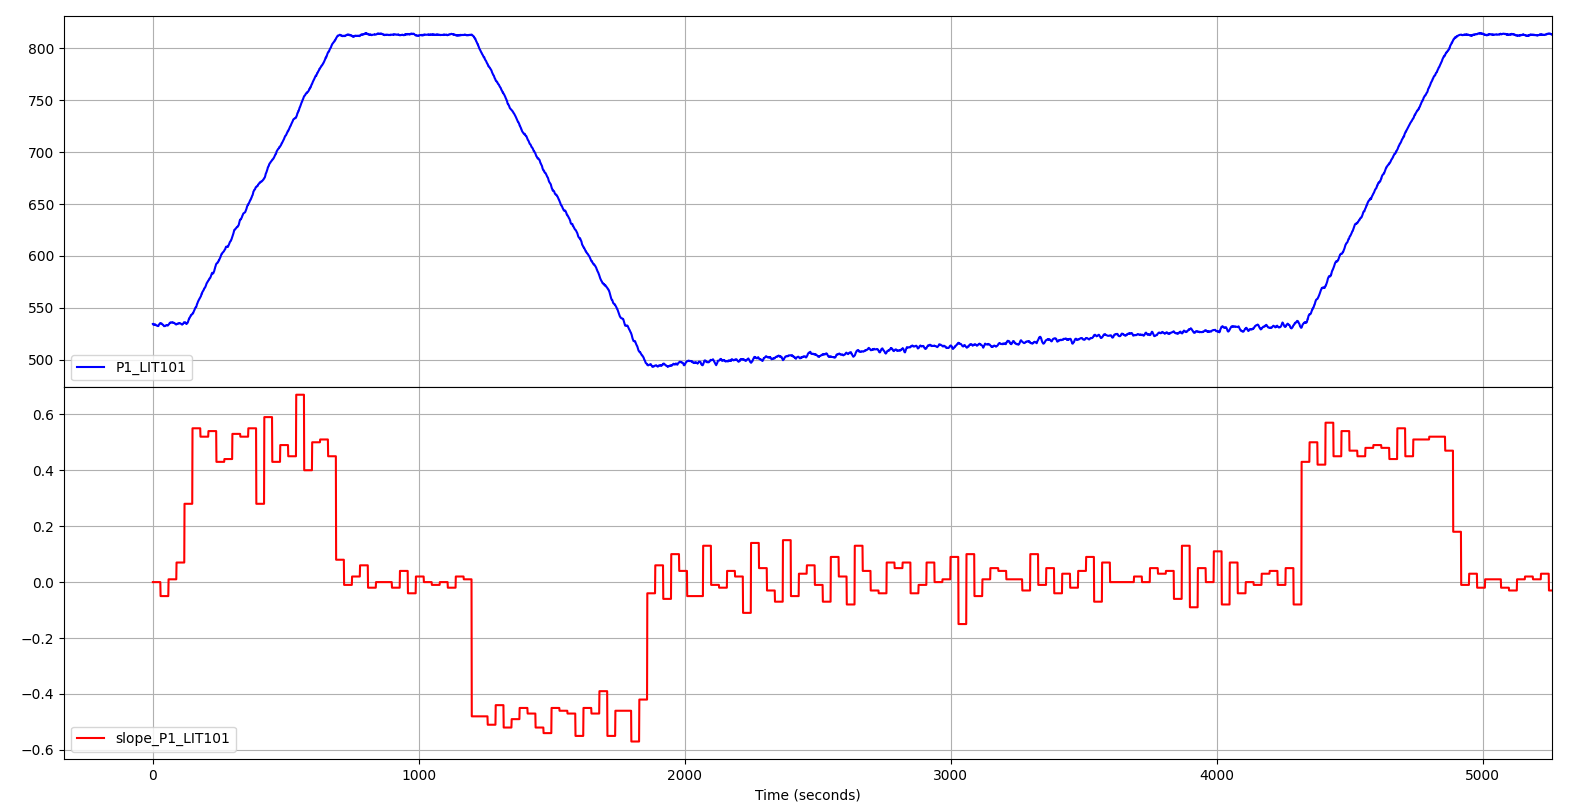
\includegraphics[width=\textwidth]{chap4/slope_nodecomp_g30_2.png}
		\caption{}
		\label{subfig:4_slope_g30_nodecomp}
	\end{subfigure}
	\hfill
	\begin{subfigure}{0.9\textwidth}
		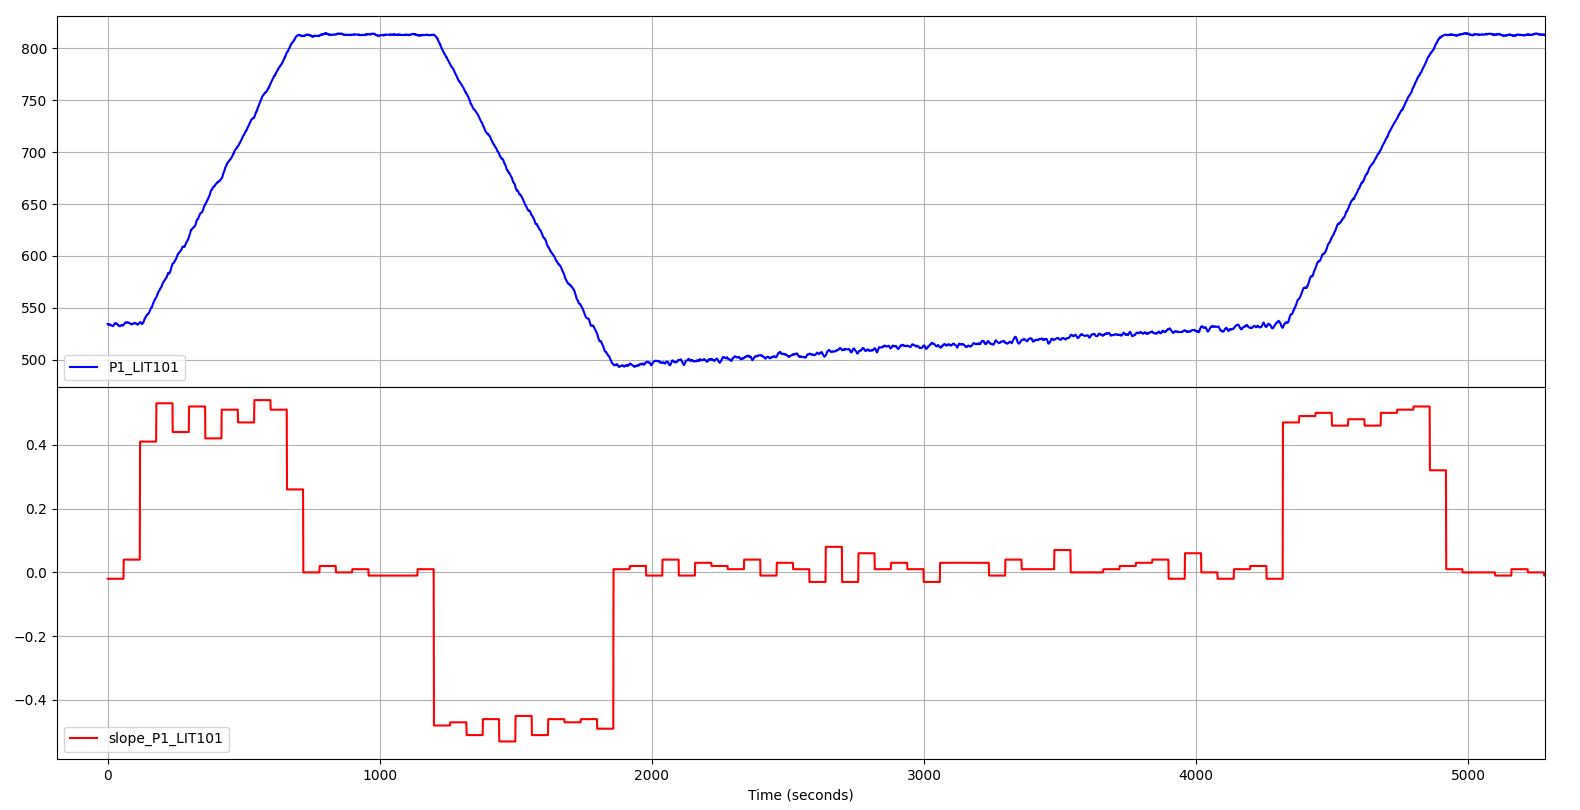
\includegraphics[width=\textwidth]{chap4/slope_nodecomp_g60_2.png}
		\caption{}
		\label{subfig:4_slope_g60_nodecomp}
	\end{subfigure}
	\begin{subfigure}{0.9\textwidth}
		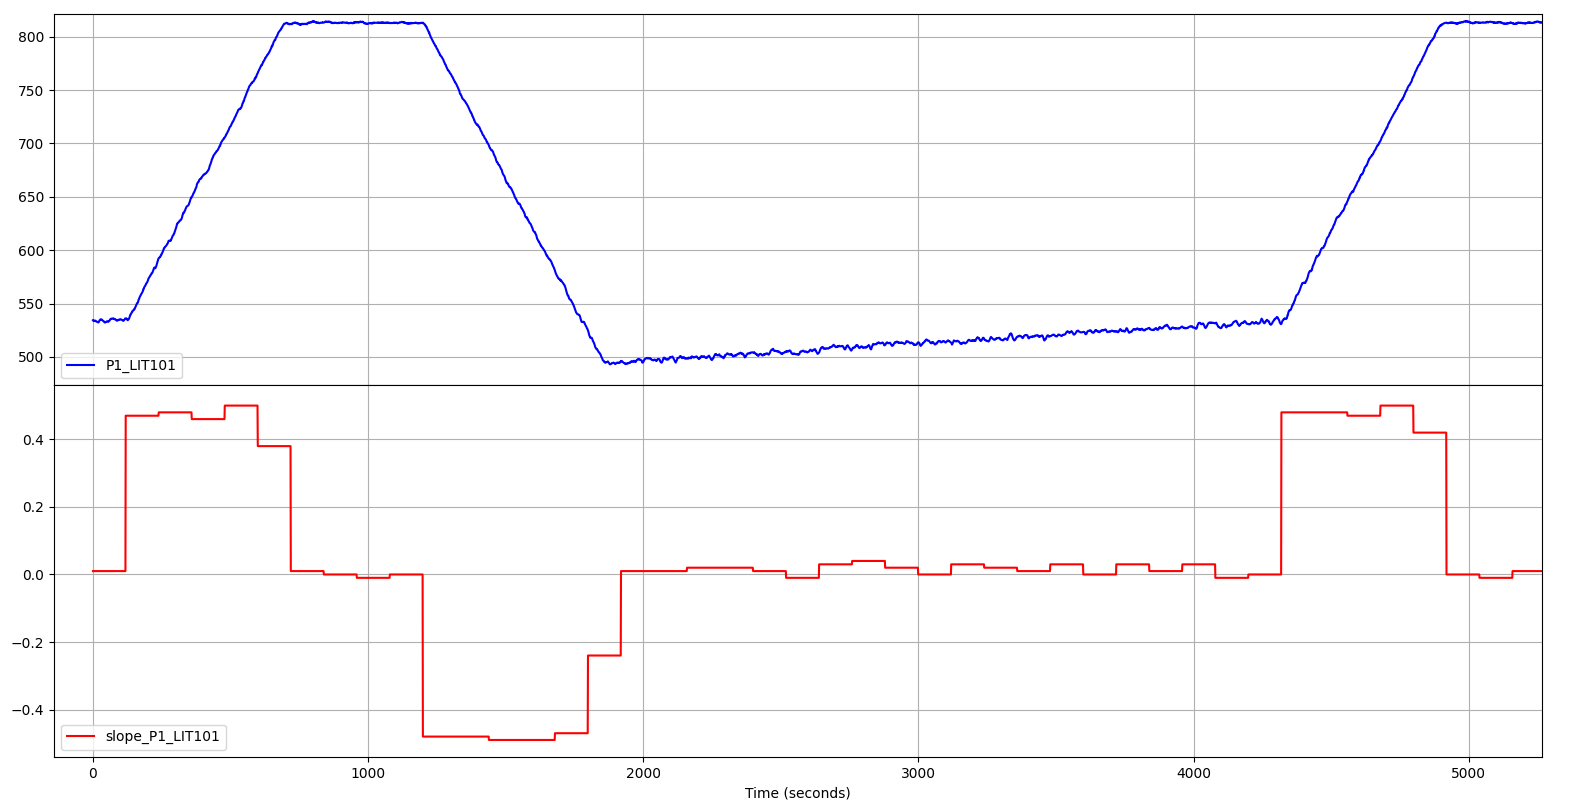
\includegraphics[width=\textwidth]{chap4/slope_nodecomp_g120_2.png}
		\caption{}
		\label{subfig:4_slope_g120_nodecomp}
	\end{subfigure}
	\caption{Slope comparison with granularity 30 (a), 60 (b) and 120 seconds (c)}
	\label{fig:4_slope_comparison}
\end{figure}

The solution to this problem is trying to remove as much "noise" as possible from the data, in order to get a more linear trend in the curve representing the measurement and consequently be able to calculate slopes more accurately.\newline
There are several ways to smooth out the noise, but two of them seemed to me to be the most suitable and that I considered and evaluated: using \textbf{polynomial regression}, thus creating a filter on the noise, or a \textbf{seasonal decomposition}, and more specifically the part concerning the \textbf{trending}.\newline
With regard to polynomial regression, I evaluated the \textit{Savitzky-Golay} algorithm \cite{savgol}, and with regard to seasonal decomposition, I evaluated \textit{Seasonal-Trend decomposition using LOESS} (STL) \cite{stl_decomp}.\newline
For reasons of the length of this paper I cannot describe these two solutions in detail (for this, I refer to the bibliographical notes): Figure \ref{fig:4_smoothing_comparison}, however, shows a quick graphical comparison of them compared with the original data. The solution chosen is the STL decomposition, which is more effective in attenuating noise than the Savitzky-Golay filter although at the cost of more delay (still present in all algorithms of this kind) in some parts.

\begin{figure}[H]
	\centering
	\begin{subfigure}{0.48\textwidth}
		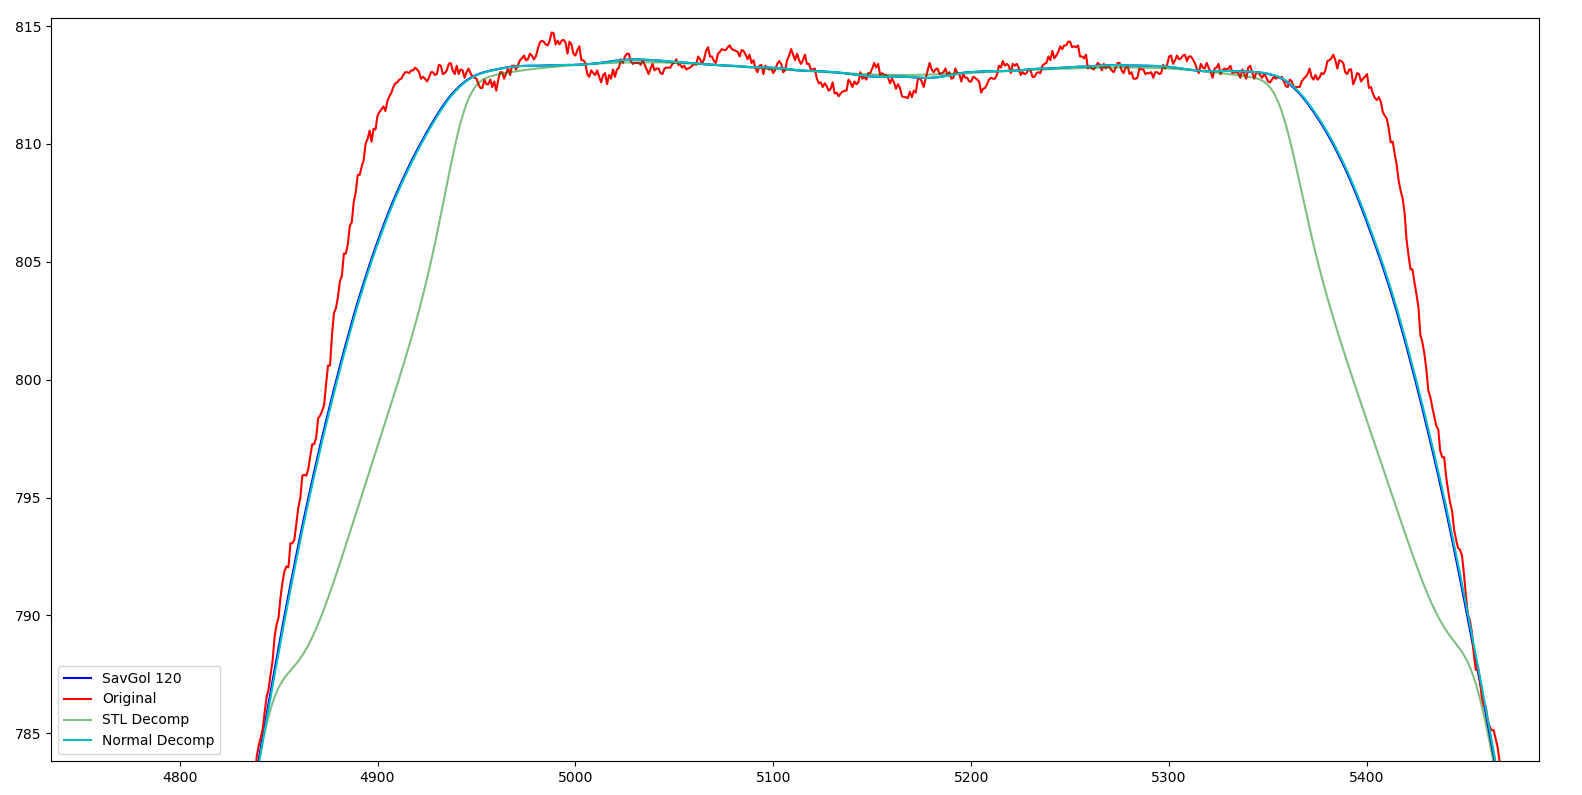
\includegraphics[width=\textwidth]{chap4/confronto_decomp_3.png}
		\caption{}
		\label{subfig:4_smoothing1}
	\end{subfigure}
	\hfill
	\begin{subfigure}{0.48\textwidth}
		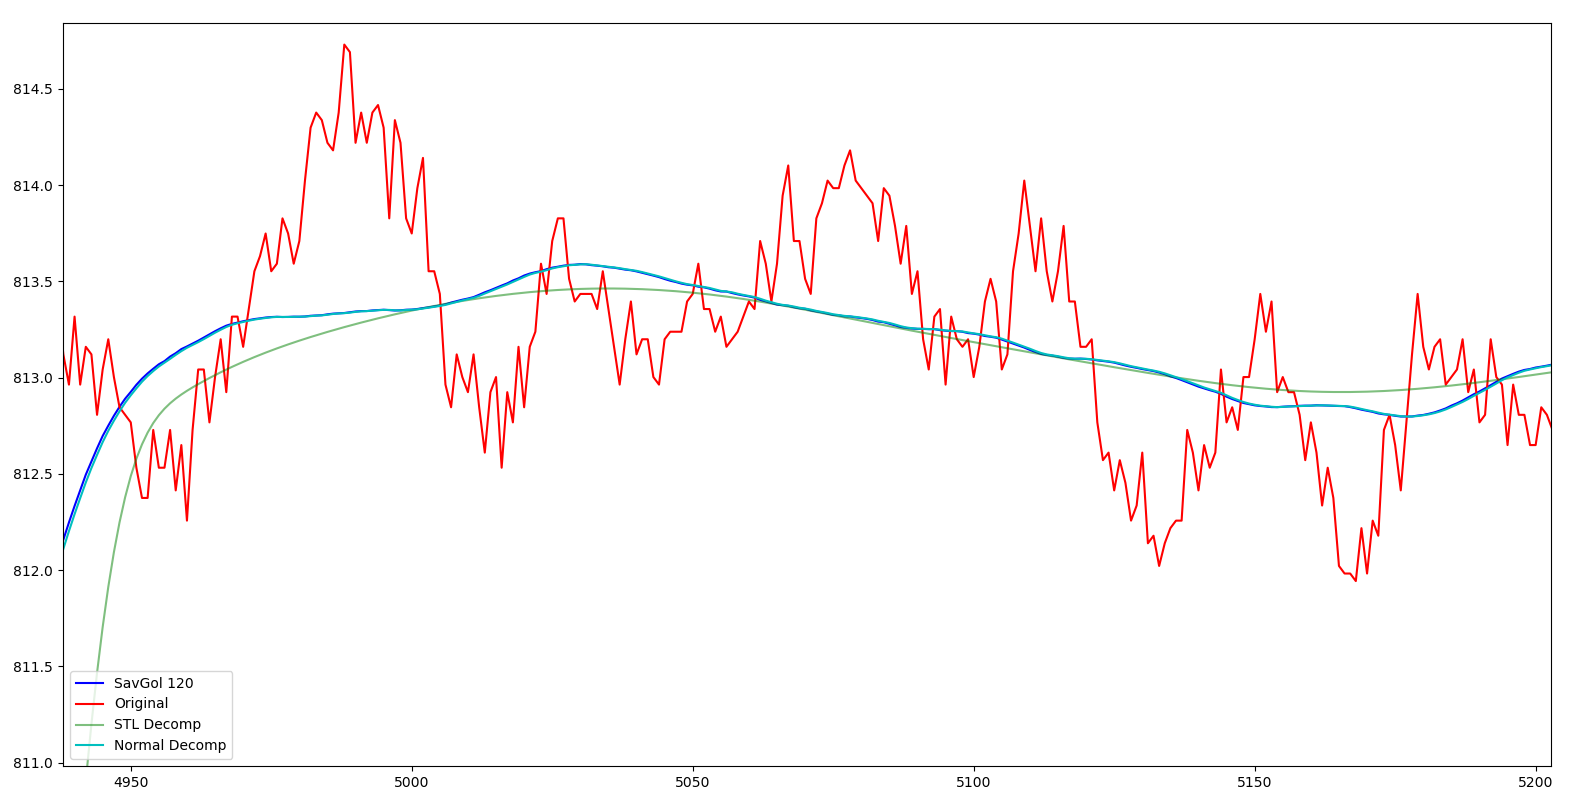
\includegraphics[width=\textwidth]{chap4/confronto_decomp_4.png}
		\caption{}
		\label{subfig:4_smoothing2}
	\end{subfigure}
	\begin{subfigure}{0.48\textwidth}
		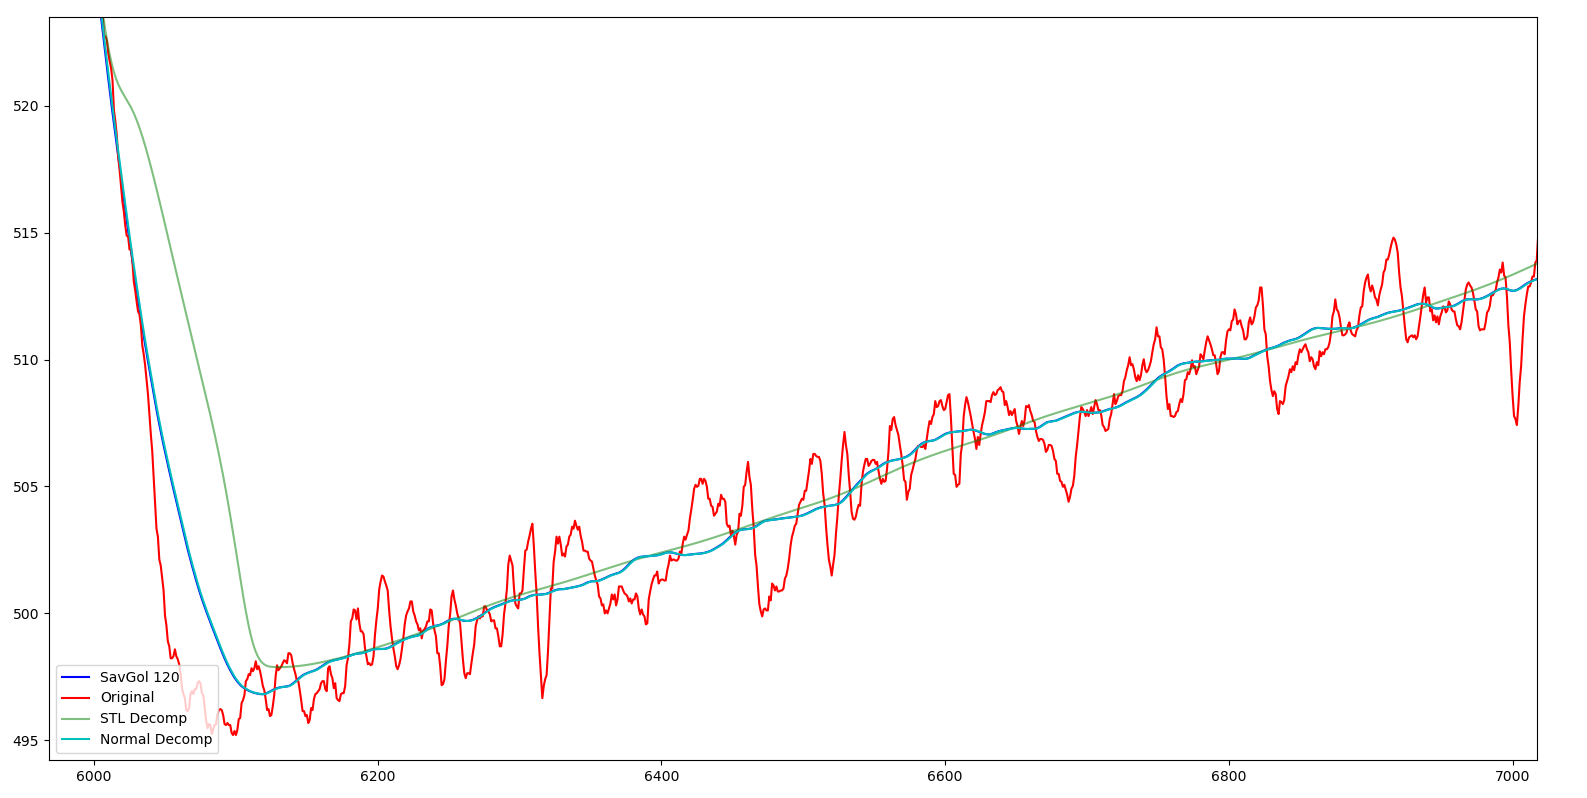
\includegraphics[width=\textwidth]{chap4/confronto_decomp_5.png}
		\caption{}
		\label{subfig:4_smoothing3}
	\end{subfigure}
	\begin{subfigure}{0.48\textwidth}
		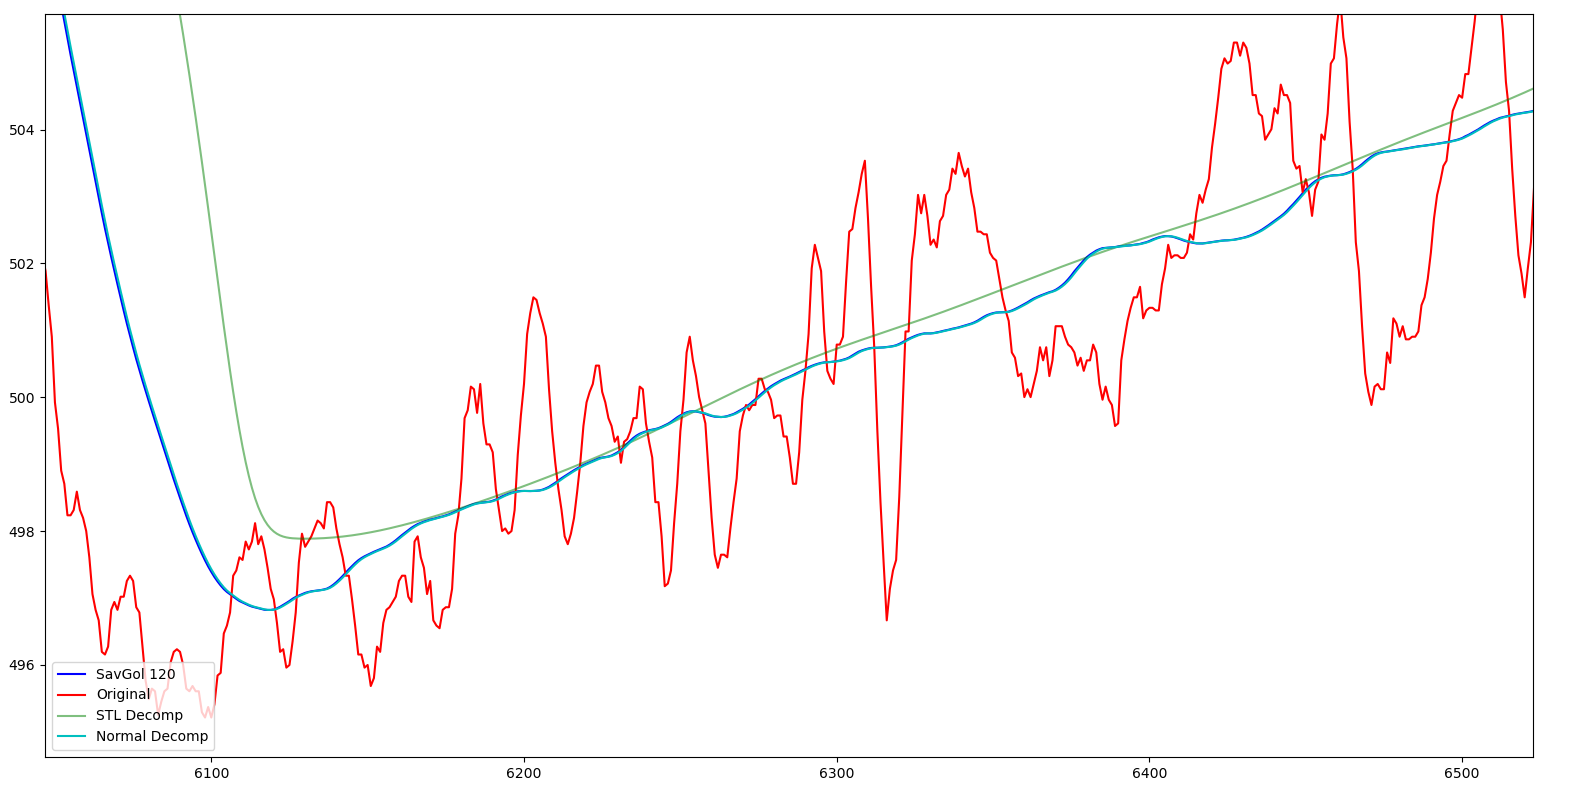
\includegraphics[width=\textwidth]{chap4/confronto_decomp_6.png}
		\caption{}
		\label{subfig:4_smoothing4}
	\end{subfigure}
	\caption{Savitzky-Golay filter (blue line) and STL decomposition (green) comparison}
	\label{fig:4_smoothing_comparison}
\end{figure}

The application of the STL decomposition results in a significant improvement in slope calculation even when using low granularity: in Figure \ref{fig:4_STL_decomp_results} it can be seen that, with the same granularity used for the example in Figure \ref{subfig:4_slope_g30_nodecomp}, the slope values, although with unavoidable fluctuations, remain within the same trend, corresponding to the trend of the data curve net of the introduced lag caused by the periodicity set for the decomposition.

\begin{figure}[ht]
	\centering
	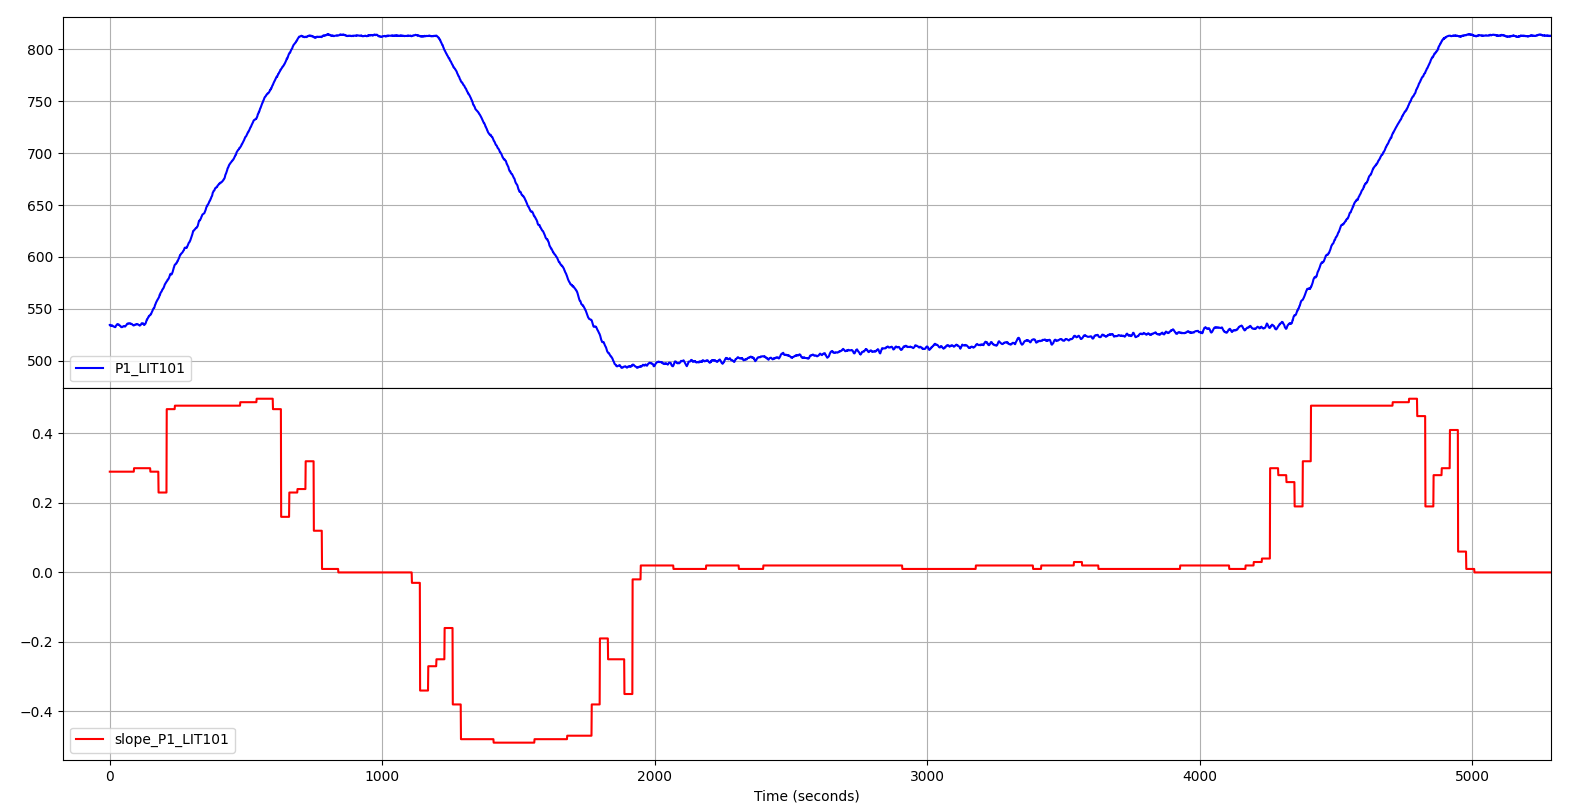
\includegraphics[scale=0.35]{chap4/slope_STL_g30_2.png}
	\caption{Slope after the application of the STL decomposition}
	\label{fig:4_STL_decomp_results}
\end{figure}
This periodicity, which indicates the sampling time window for decomposition and thus the level of noise smoothing, can be set in the \textit{config.ini} configuration file in the \texttt{trend\_period} directive.\newline
The slope calculation will then be performed on the data from the additional measurement trend attributes specified in the \texttt{trend\_cols\_list} directive in the configuration file, and no longer on the original unfiltered data.

\bigskip
Finally, to enable Daikon to correctly interpret the slope data, the decimal values corresponding to each calculated slope are converted into three numerical values -1, 0, and 1, which correspond to the decreasing (if the slope is less than zero), stable (if it is equal to zero), and increasing (if it is greater than zero) trends, respectively. In Figure \ref{fig:4_slope_daikon}, the new slope can be seen, along with the curve obtained from the STL decomposition:

\begin{figure}[ht]
	\centering
	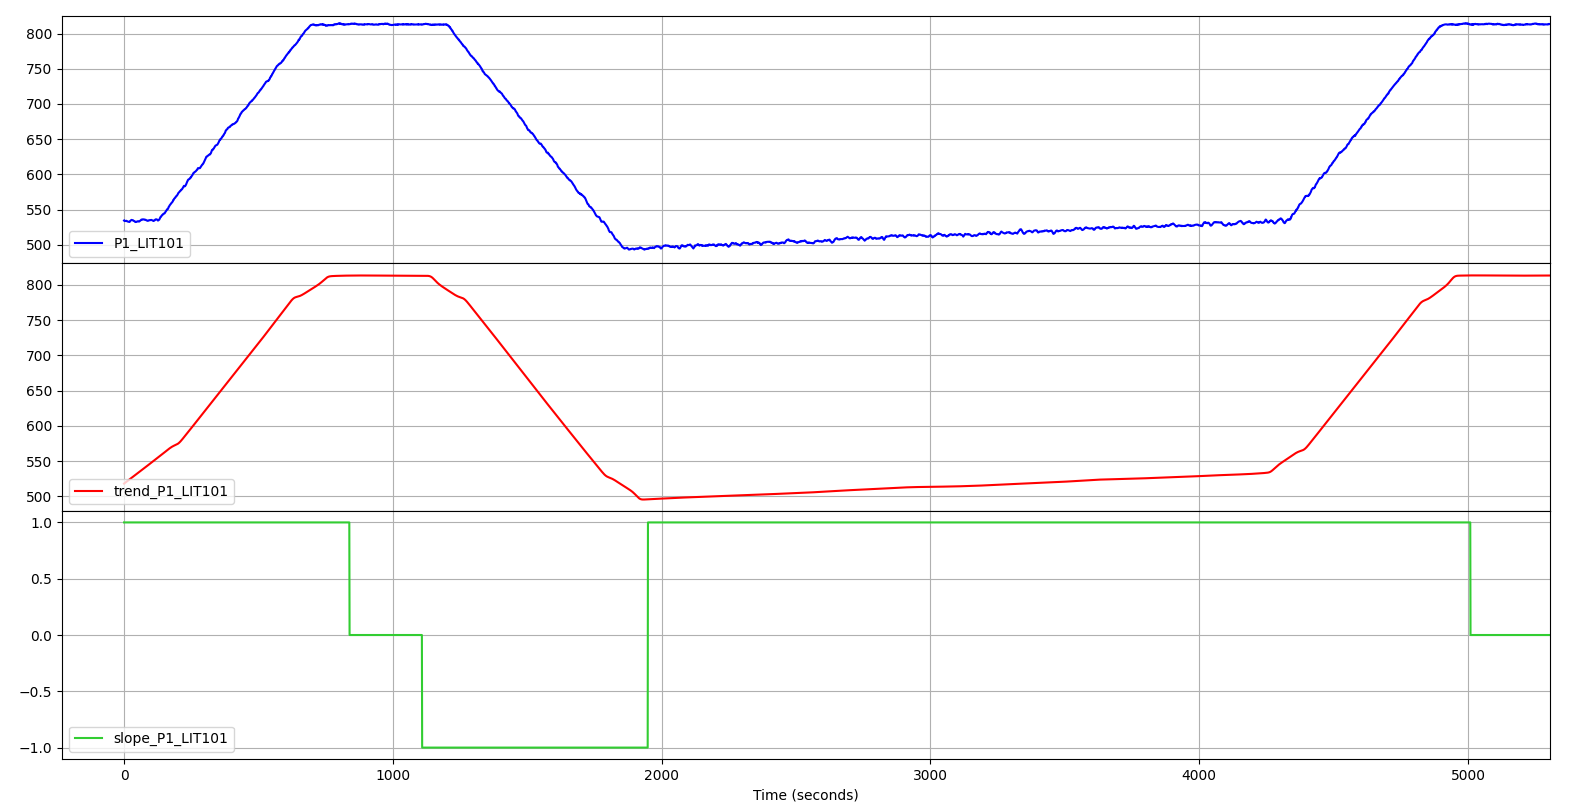
\includegraphics[scale=0.35]{chap4/slope_STL_bin_g30_2b.png}
	\caption{The new slope representation (green line) and the smoothed measurement data obtaind with the STL decomposition (red)}
	\label{fig:4_slope_daikon}
\end{figure}

\subsubsection{Datasets Merging}
\label{subsubsec:4_dataset_merging}
In this step the individual datasets are merged, obtaining two new distinct datasets: one without the enrichment and that will be use in the process mining phase, and the other, containing the additional attributes but with the timestamp column removed, intended for inference and invariant analysis.

\bigskip
The first of the two datasets obtained will be saved in CSV format by default in the \texttt{\$(project-dir)/process-mining/data} directory while the second one in the \texttt{\$(project-dir)/daikon/Daikon\_Invariants} directory (both paths are however configurable via \textit{config.ini}).\newline
The dataset name is specified in \textit{config.ini} or via the \texttt{-o} command-line option: in the case of the dataset intended for process mining, the script will automatically add a \texttt{\_TS} suffix to the filename, indicating the fact that the dataset includes the timestamp.\newline
The opportunity for the user to specify a different filename for the output each time allows the user to save the execution trace of the selected subsystem without overwriting the previous ones and thus to use all of them in the subsequent phases of the analysis.

\subsubsection{Brief Analysis of the Obtained Subsystem}
\label{subsubsec:4_brief_analysis}

At the end of the datasets merging and saving step, the user is asked whether to perform a brief optional analysis of the final resulting dataset to extract preliminary data, with the purpose of obtaining basic information about the (sub)system and possibly refining the enrichment.\newline
If the user responds affirmatively to the request, \texttt{mergeDatasets.py} launches within it a further Python script located in the same\\ \texttt{\$(project-dir)/pre-processing} directory, called \texttt{system\_info.py}. This script, using a combination of Daikon and Pandas analysis, performs a quick analysis of the dataset contents trying to \textbf{recognize}, however roughly, \textbf{the register types}, with possible maximum and minimum values and hardcoded setpoints. In addition, using the additional attribute \texttt{prev\_}, it is capable of deriving measurement values in correspondence with state changes of individual actuators.\newline 
Listing \ref{lst:4_brief_infos} shows an example of this brief analysis elated to PLC1 of the iTrust SWaT system (for brevity, only one measurement is reported in the analysis of actuator state changes):

\begin{lstlisting}[language=bash,numbers=none,caption={Example of preliminar system analysis},label=lst:4_brief_infos]
	Do you want to perform a brief analysis of the dataset? [y/n]: y
	
	Actuators: 
	P1_MV101 [0.0, 1.0, 2.0]
	P1_P101 [1.0, 2.0]
	
	Sensors: 
	P1_FIT101 {'max_lvl': 2.7, 'min_lvl': 0.0}
	P1_LIT101 {'max_lvl': 815.1, 'min_lvl': 489.6}
	
	Hardcoded setpoints or spare actuators: 
	P1_P102 [1.0]
	
	       P1_LIT101  P1_MV101  prev_P1_MV101
	669     800.7170         0              2
	1850    499.0203         0              1
	4876    800.5992         0              2
	6052    498.9026         0              1
	9071    800.7170         0              2
	10260   499.1381         0              1
	13268   801.3058         0              2
	14435   498.4315         0              1
	17423   801.4628         0              2
	18603   498.1567         0              1
	
	P1_LIT101  P1_MV101  prev_P1_MV101
	677     805.0741         1              0
	4885    805.7414         1              0
	9079    805.7806         1              0
	13276   805.1133         1              0
	17432   804.4068         1              0
	
	P1_LIT101  P1_MV101  prev_P1_MV101
	1858    495.4483         2              0
	6060    497.9998         2              0
	10269   495.9586         2              0
	14443   495.8016         2              0
	18611   494.5847         2              0
	
	       P1_LIT101  P1_P101  prev_P1_P101
	118     536.0356        1             2
	4322    533.3272        1             2
	8537    542.1591        1             2
	12721   534.8581        1             2
	16883   540.5890        1             2
	
	P1_LIT101  P1_P101  prev_P1_P101
	1190    813.0031        2             1
	5395    813.0031        2             1
	9597    811.8256        2             1
	13776   812.7283        2             1
	17938   813.3171        2             1
\end{lstlisting}

From these results we can see that: 

\begin{itemize}
	\item the probable actuators are \texttt{P1\_MV101}, which assumes three states identified by the values 0, 1 and 2, and \texttt{P1\_P101}, which instead assumes two states identified by the values 1 and 2
	
	\item there are two probable measures: \texttt{P1\_FIT101} whose values range from 2.7 to 0.0, and \texttt{P1\_LIT101} whose values range from 815.1 to 489.6. One conjecture could already be made about the topology of the system: \texttt{P1\_LIT101} represents a tank
		
	\item apparently there are no related \textit{hardcoded setpoints}, but a probable spare actuator, \texttt{P1\_P102}, whose value is always 1. From this data, another conjecture can be made: the value 1 is the close state for that particular type of actuators, while 2 represents the open state
	
	\item from the analysis of state changes, in summary, we derive some \textit{relative setpoints}: for example, we know that \texttt{P1\_P101} changes state from value 1 to value 2 when the level of \texttt{P1\_LIT101} is about 813, while it changes from value 2 to 1 when the level of \texttt{P1\_LIT101} is about 535. We can deduce that \texttt{P1\_P101} is responsible for emptying the tank	
\end{itemize}

The information obtained here can be used, as mentioned above, to refine the enrichment of the dataset by setting directives in the \texttt{[DATASET]} section of the \textit{config.ini} file, should this be empty or only partially set, or to make the first conjectures about the system, as we have just seen.

\bigskip
The \texttt{system\_info.py} file can also run in standalone mode if needed: it takes as command-line arguments the dataset to be analyzed, a list of actuators, and a list of sensors. For analysis related to state changes, the dataset must mandatorily be of the enriched type.

\subsection{Phase 2: Graphs and Statistical Analysis}
\label{subsec:improve_graphs}

The new \textit{graph analysis} arises from the need to give the user an overview of the (sub)system obtained in the previous pre-processing phase, identifying more easily the typology of the registers and grasping more effectively the relationships and the dynamics that may exist between the registers controlled by one or more PLCs, confirming the initial conjectures if the brief analysis described in the previous section has been performed, or making new ones thanks to the visual graph support. 

\bigskip
In the previous tool, as already pointed out in Section \ref{subsec:ceccato_limitations}, it is possible to view the chart of one only register at a time: this certainly makes it possible to identify, or at least to hypothesize, the type of that register, but it makes it very complicated to be able to relate it to the other components of the system and thus to derive conjectures about the behavior of the latter, conjectures to be possibly confirmed in the later phases. Hence the need to create a tool that was better than the previous one and that provided more information in an easier way.

\subsection{Phase 3: Invariant Analysis}
\label{subsec:improve_invariants}

%\subsection{Automatic Detection of Actuators and Sensors}
\subsubsection{Invariants Generation}

\subsection{Phase 4: Businness Process Analysis}
\label{subsec:improve_bpa}

%\section{Extra Information on the Physics}
%\label{sec:extra_info}

\vfill
\nolinenumbers